%%% Thesis Introduction --------------------------------------------------
\chapter{INTRODUCTION}
\label{chap:intro}
\graphicspath{{Introduction/IntroductionFigs/EPS/}{Introduction/IntroductionFigs/}}
\nomenclature[z1]{$CMS$}{Character Motion Synthesis}


\section{The Challenge}
Character Motion Synthesis (\cms) research aims at generating motions for virtual characters.
It is a valuable topic for both industry and academic community. 
Besides the main applications in the media industry, where both computer games and animation films depend heavily upon character motions for storytelling;  
CMS also has applications in many different areas, such as user interface design, psychology, sports and medicine.

The challenge of CMS research is not to make characters move, but how to make them lifelike. 
Underlying this is our human's marvellous ability of motion perception. 
In fact, motions are very similar; 
while from the varieties in motion details, humans can infer the changes in mental states, health conditions or the surrounding environment.
\note{uncanny valley}
A famous phenomon about motion perception properties is the ``uncanny valley''.
For characters with realistic humanlike appearance, slightly artefacts in motions may result a big drop in human likeliness.



Nowadays in industry, high quality motions are mainly generated by manual work. 
In applications, most characters are very complicated and contain a large number of joints, making animation a tedious work.
Making it worse, reusing motion animation is also difficult and prone to artefacts.
For this situation, high level animation tools are badly needed. 

\note{Do An introduction for physicall based animaiton?}
Current Research focuses on physics based CMS, expect it will eliminate the artefacts from violating physics and add motion response to dynamic perturbation.
Currently,this paradigm faces many difficulties such as computational cost and modelling complexity.

this problem is spotted by researchers from diffferent areas in different perspectives.
Underlying the ``uncanny valley '' is the question how we perceive motor dynamics.
We don’t judge motion by check the physics validity.
Some awkward artefacts are spotted instantly even they are physically feasible, while many physical impossible motions are accepted as enjoying. 

How we perceive the world is foudation how we move in it.
The oddity of perception and dynamic motor control may suggests our neural system adopted a totally different paradigm for dynamic perceiving and motor control.
Difficulties in \cms mainly comes from the inferiority of our artificial control techniques.
By exploring possible new paradigms, in this thesis, we propose new ideas for motion perception and motor control.

 

\section{Agile Animals}
%\note{Underlying these problems} is our misunderstanding of animal motions.
Although animals have fancied us for thousands of years, we still don't fullly understand how they move and how we perceive their motions.
Animals move in a different way than artificial machines.
Investigations in differences between machines and animals may provide us with an in-depth understanding of questions facing nowadays CMS researchers.
%some basic questions of motor control and motion perception remain open. 
%And answers to such questions become even more valuable nowadays. 
%Advance in this topic will greatly influence the biology, robotic engineering even intelligent research.
\note{The difference between biological motor system}

%The paradoxes is even human are good at motor control and motion perception; human still don’t have an idea of how we move and how we perceive motion.
%Before going into details into the research ideas, we first review some puzzles troubles the foundation of CMS. 
\begin{itemize}
\HiItem {Degrees of freedom (DOFs)}.
From Mechanical point of view, the first distinction is the huge gap in DOF counts. 
Biological systems have much more DOFs than their artificial counterparts.
An artificial ship can be approximately modelled as a rigid body; while the flexible vertebrae of fishes is composed of tens of DOFs.


In principle, extra DOFs provides more types of variations and adaptations for motions. 
But from the control perspective, extra DOFs complicate the motion control task. 
For the human example, neural system controls more than 600 muscles to take one step.
For CMS research, the extra DOFs are redundant and become the ``{\dof}s Curse''.
 
\HiItem {Versatility}
Most artificial machines are designed with a single purpose.
While animals are able  for many more tasks.
For example, beside the walking, swimming and many styles of locomotion , human  use a large number of tools for motion tasks, such as driving a car, skating, cycling, and playing tennis.
CMS researchers may negalect that behaviour the feeding, breeding, language, vision all depends on motions and motor control. 

Follos the question how much resources is allocatted for motor control.

\HiItem{Performance}
Even motor control is more complex for animals, the outcome performance surpass artificial machines in many aspects.
natural motion are more
\begin{enumerate} 

\HiItem{robust}
Human maintain walking stability on tough terrain unaccessible for vehicles.

\HiItem{maneuverability and speedy}
Typical modern airplanes will travel about $32 body lengths/sec$ and rotate $720 deg/sec$.
while pigeon may travel $75 body length / sec$, rotate more than $5000deg/sec$.

\HiItem{Energy Efficient}
An example is the energy consumed by human walking is only $5\%$ of that for the world famous robot ASIMO.
\end{enumerate}

\end{itemize}



%For computer animation research, the key principle is we should know the things we animate.
%Natural motion system has many valuable properties which are not captured by current motion synthesis methods.
%\begin{itemize} 
% \HiItem{robust}
%Natural motions are adaptive to the changes in the environment or body conditions. 
%A common example is human locomotion. 
%Walking on different terrains will exhibit different gait while the balance is maintained. 
%
%\HiItem{speedy}
%Some motions of animals are very fast, honey birds may vibrate their wings in kHz.
%The astonishment is to the speed of motion, more puzzling is that the neural system can solve the complex motion control problem in such a short time. 
%When an animal avoids obstacles at very high running speed, 
%it must continue its running, make a turning and keep balance at the same time. 
%It seems easy for the neural system to plan complicate motions.
%\HiItem{Energy Efficient}
%Natural Motions are energy efficient.
%In theory, this idea is supported by Darwin's Theory of Evolution.
%But animals spent far less energy than our expectation.
%An example is that the energy consumed by human walking is only 5\% of that for a robot of the same scale.
%\end{itemize}


\section{Different Ideas}
Our method is different in many different ways from current paradigms.
Comparing them side by side will provides a clearing understaning of the difference. 

\begin{itemize}
\HiItem {Control Function Model}
The first question is by which mean we control our motor ability.
Some researchers supported the idea motor control based on computation or our reasoning power.
In \cms , this is procedure paradigm.
The redundant {\dof}s spoils this paradigm with computational burden.
Pure procedures methods are impossible to run in realtime.

Facing this problem, some researchers support the idea motor control are memory based.
In \cms, this is the datadriven paradigm.
It is the versatality and adaptativity that made this paradigms problemistic.
Unlimited memory for data is needed and searching in ever increasing database becomes more and more challenging.

The foundation idea of our research is different.
We support the idea that motions are ``easy '' and don't need big effort to control.
It is the body and environment play the crucial role in motion, they form the basic templates for many motion tasks.
Neural System only tweaks the basic templates for specific purpose.



 
 
	
\HiItem{Control Strategy}
The second question is the control strategy.
Most Artificial system are control by the paradigms of feedback.
Usually the motion is planned first and control is applied to counter act perturbations.
Current \cms follows the idea and the method is called ``shooting''.


The control strategy of our research is different and belongs to feed forward category.
The purpose of control is make motions ``easier'', if perturbations are expected, measures are taken beforehand to prevent ``failure'' of motion.
Also details of motion are uncontrolled, only the final result is concerned.


\HiItem{Attitude of Natural Dynamics}
The biggest difference is the attitudes of natural dynamics. 
Many \cms research plan the motion before execute motion.
The natural dynamics effects of the body are treated as perturbation and canceled by control input.


The mechanical system of animals evolve with the enivronment, it is the product of natural selection of millions of years.
We treat the natural dynamics as a heritage rather than a burden. 
In our research, we limit the control input and explore the natural dynamics to maintain the natural-looking features.
\end{itemize}


\section{Examples For Motor Invariant Theory}
%In this thesis, we propose different idea towards motor control and motion synthesis.
%In this research, we propose a different motion synthesis method based on a different motor control theory.
%
%An insightful discovery is that motor control can be “easy”.
%For some situation, some tasks mainly explore the properties of the body and environment and can be achieved with little control effort.
%In nature, we don’t finish difficult motion tasks, we select many easy motion tasks that we are good at, connect or modify them for our special purpose.
%
%The “easy” tasks are called motion primitives; they are the basic elements of our motor ability. 
%When we modify the motion primitives, some valuable properties of motion primitives are kept unchanged, and the maintained properties are called motor invariants.
%
%The inspiration of our idea comes from related biological research, which covers biomechanics and neural science.

New mathematical tools are introduced to develope control techniques for our motor control.
Key problems include how to identify and modeling the tweaking of basic motion templates.





Although some obscure knowledge is needed to for the mathematical model, the principle is illustrative through some daily example. 
Here provides two examples about our idea of the ``easy'' motion and how can we “tweak” them.

The world is complex, the first question is how much information we need for accomplish a motor task. 
Our discovery that some motion task is so easy that e we need no control effort and blindness to some information doesn’t matter.
This idea is illustrate by the ship floating example

\subsection{Ship Floating}


\subsubsection*{Dynamics}
The first example is the ship floating. 
In real life, usually the height of the ship is much larger than the width. 
When wave comes, also comes the question how the ship maintains its posture.
To our surprise, we find maintain posture is “easy”.



\begin{figure}[!htbp]
  \begin{center}
    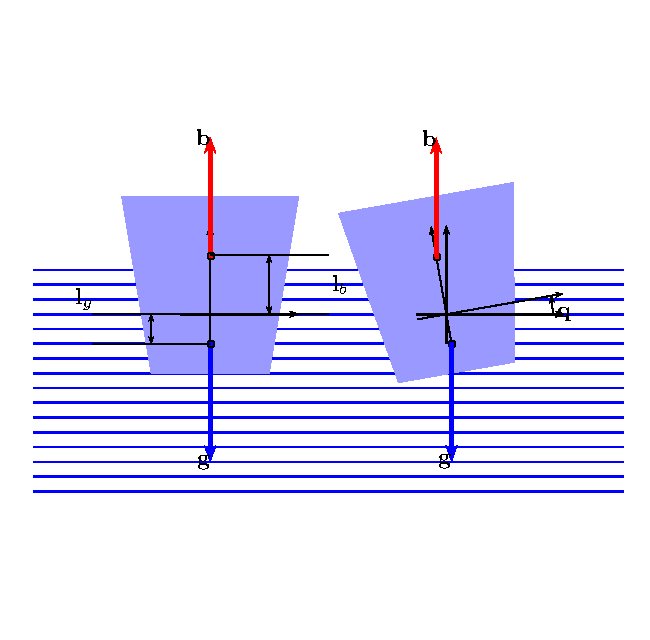
\includegraphics{ShipExample}
    \caption{Floating Ship Example}
    \label{fig:ShipFloating}
  \end{center}
\end{figure}



The side sway motion as shown in Figure ~\ref{fig:ShipFloating} is described by the dynamic ~\ref{eq:shipflow}
\begin{equation}
I_{netia}\ddot{q}+d\dot{\theta}=T_{G}+T_{B}+T_{F}=(Gl_{g}-Bl_{b})sin(\theta)+T_{F}
\label{eq:shipflow}
\end{equation}
$q$ is the swaying angle,
$I_{netia}$ is the inertia,  
$d$ is the damping coefficient,
$T_{G}$ is the torque of gravity, and $T_{B}$ is the Torque of buoyancy.
$T_{F}$ is the external control torque.
if $T_{F}=0$, external control force is applied, the system is an \textbf{autonomous system}.





\subsubsection*{Equilibrium Posture}
Ship will only rest at postures when external torqueses are zero.
There are only two postures that the external torque is zero as show in Figure ~\ref{fig:ShipEqulibrium}
\begin{figure}[!htbp]
  \begin{center}
    \leavevmode
      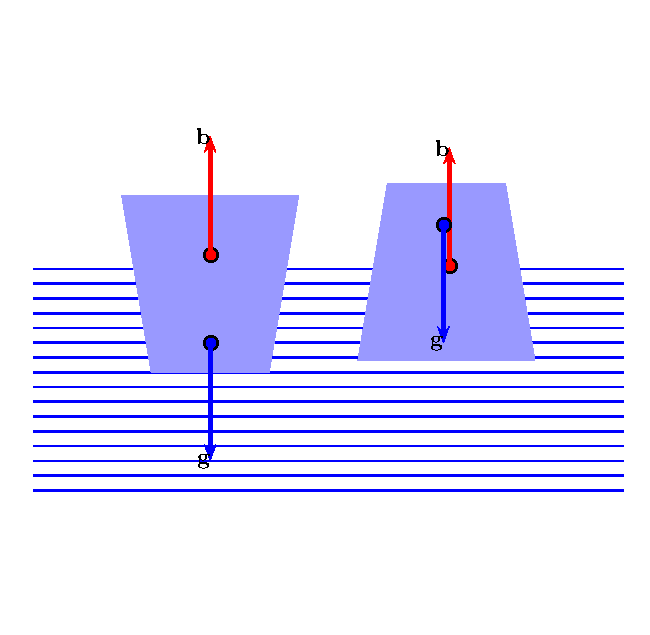
\includegraphics{ShipEquilibrium}
    \caption{Two Equilibrium Posture}
    \label{fig:ShipEqulibrium}
  \end{center}
\end{figure}



The two postures are qualitative different.
The left posture is attractive, if small perturbation moves the ship away from the left equilibrium posture, then it will return to equilibrium posture.

The right posture is repelling.
If a small perturbation moves the state of the ship away from the equilibrium posture, it will move away from the posture.

The differences of the two postures can be illustrated with the \textbf{phase plot}.
On phase plot, x axis is the angle, y axis is the angle velocity. 
Then the movement of the ship can be presented by a curve.
Figure~\ref{fig:StablePosture}  shows motion about the left equilibrium posture, they will automatically move to the left equilibrium posture.
Figure~\ref{fig:unStablePosture} shows the ship motion about the right equilibrium posture.
 
\begin{figure}[!htbp]
  \begin{center}
    \leavevmode
    \ifpdf
      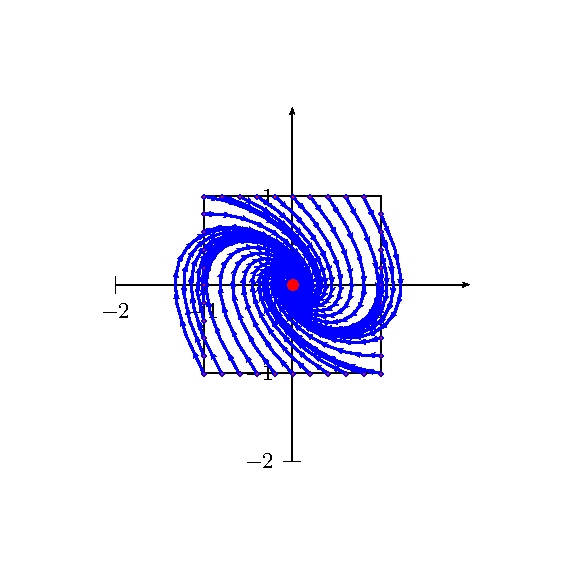
\includegraphics[height=6in]{stablePosition}
    \else
      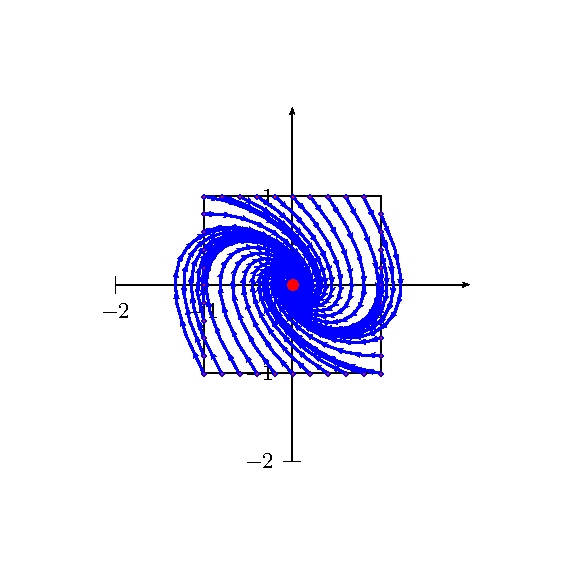
\includegraphics{stablePosition}
    \fi
    \caption{StablePosture}
    \label{fig:StablePosture}
  \end{center}
\end{figure}


\begin{figure}[!htbp]
  \begin{center}
    \leavevmode
    \ifpdf
      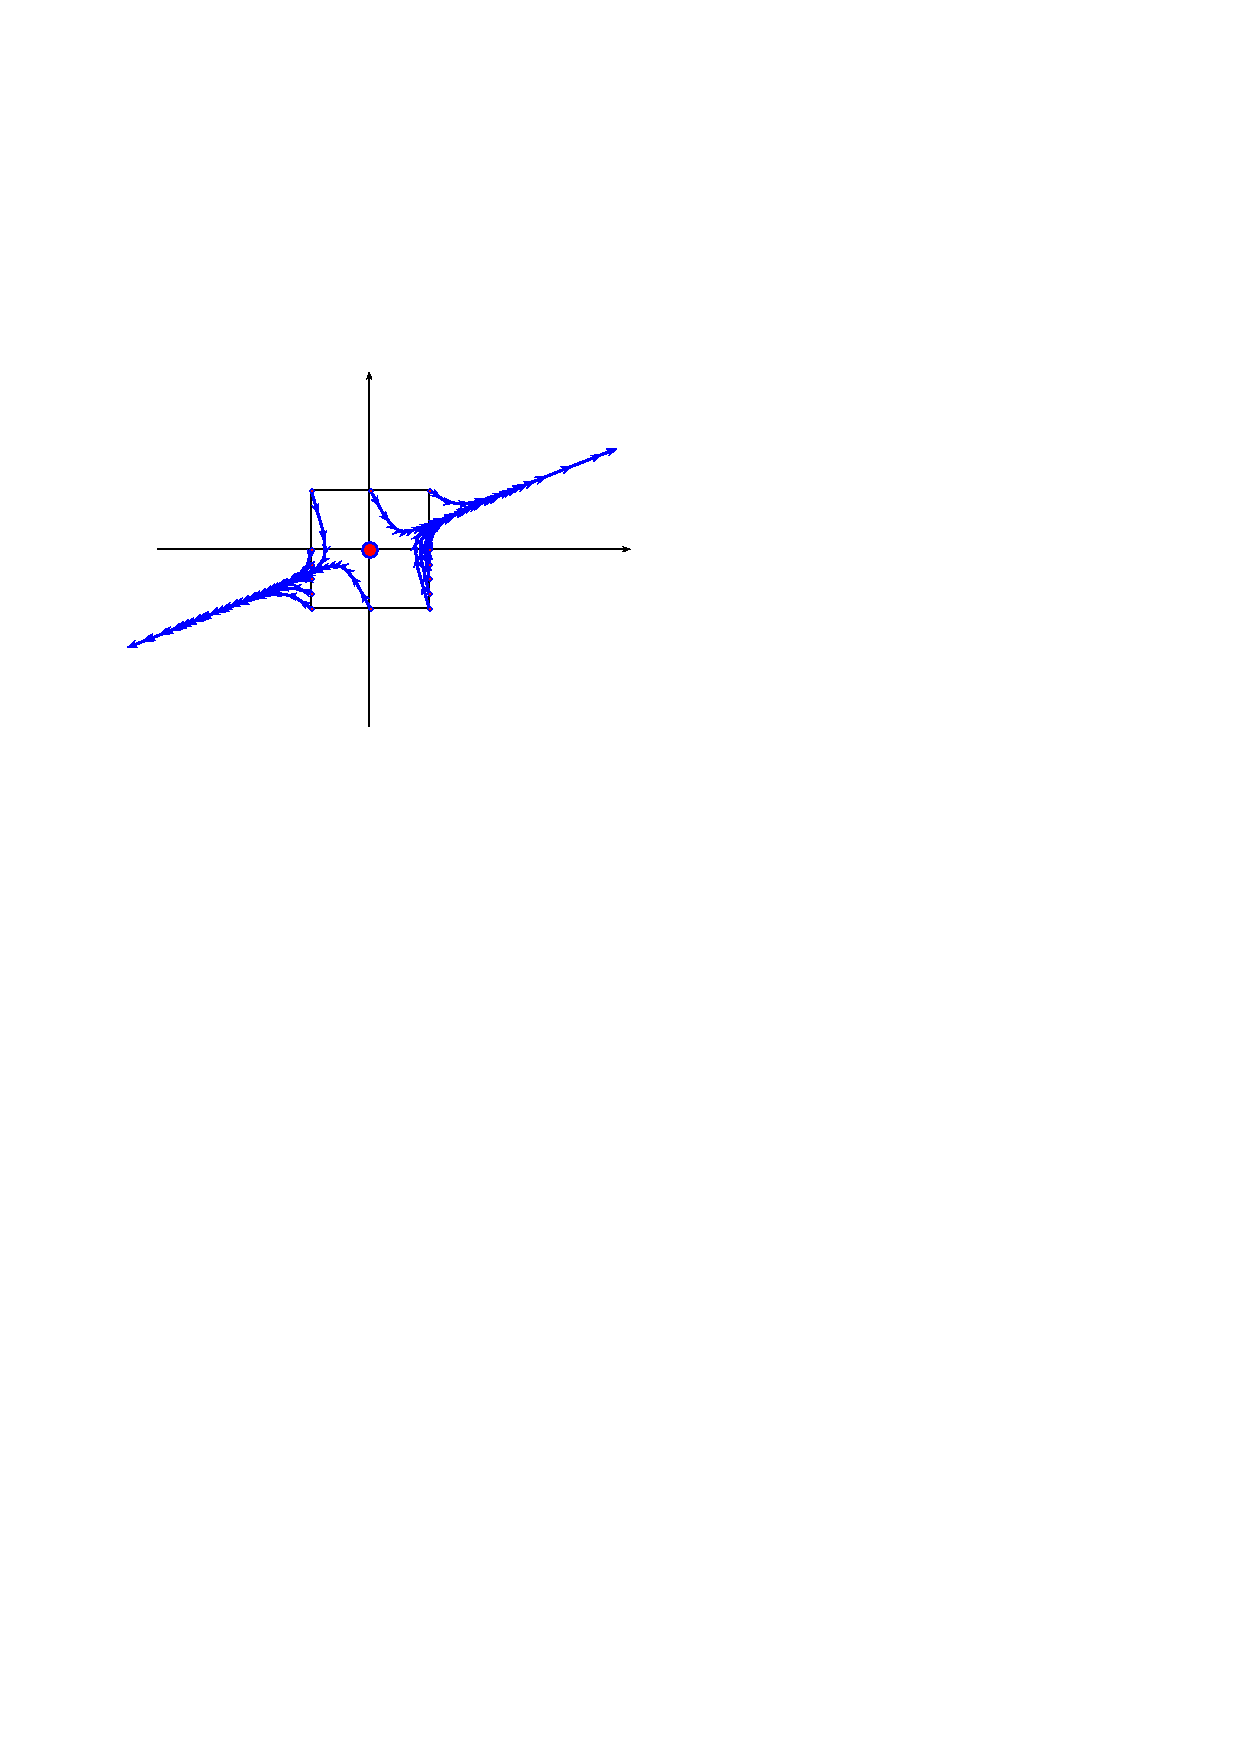
\includegraphics[height=6in]{unstablePosition}
    \else
      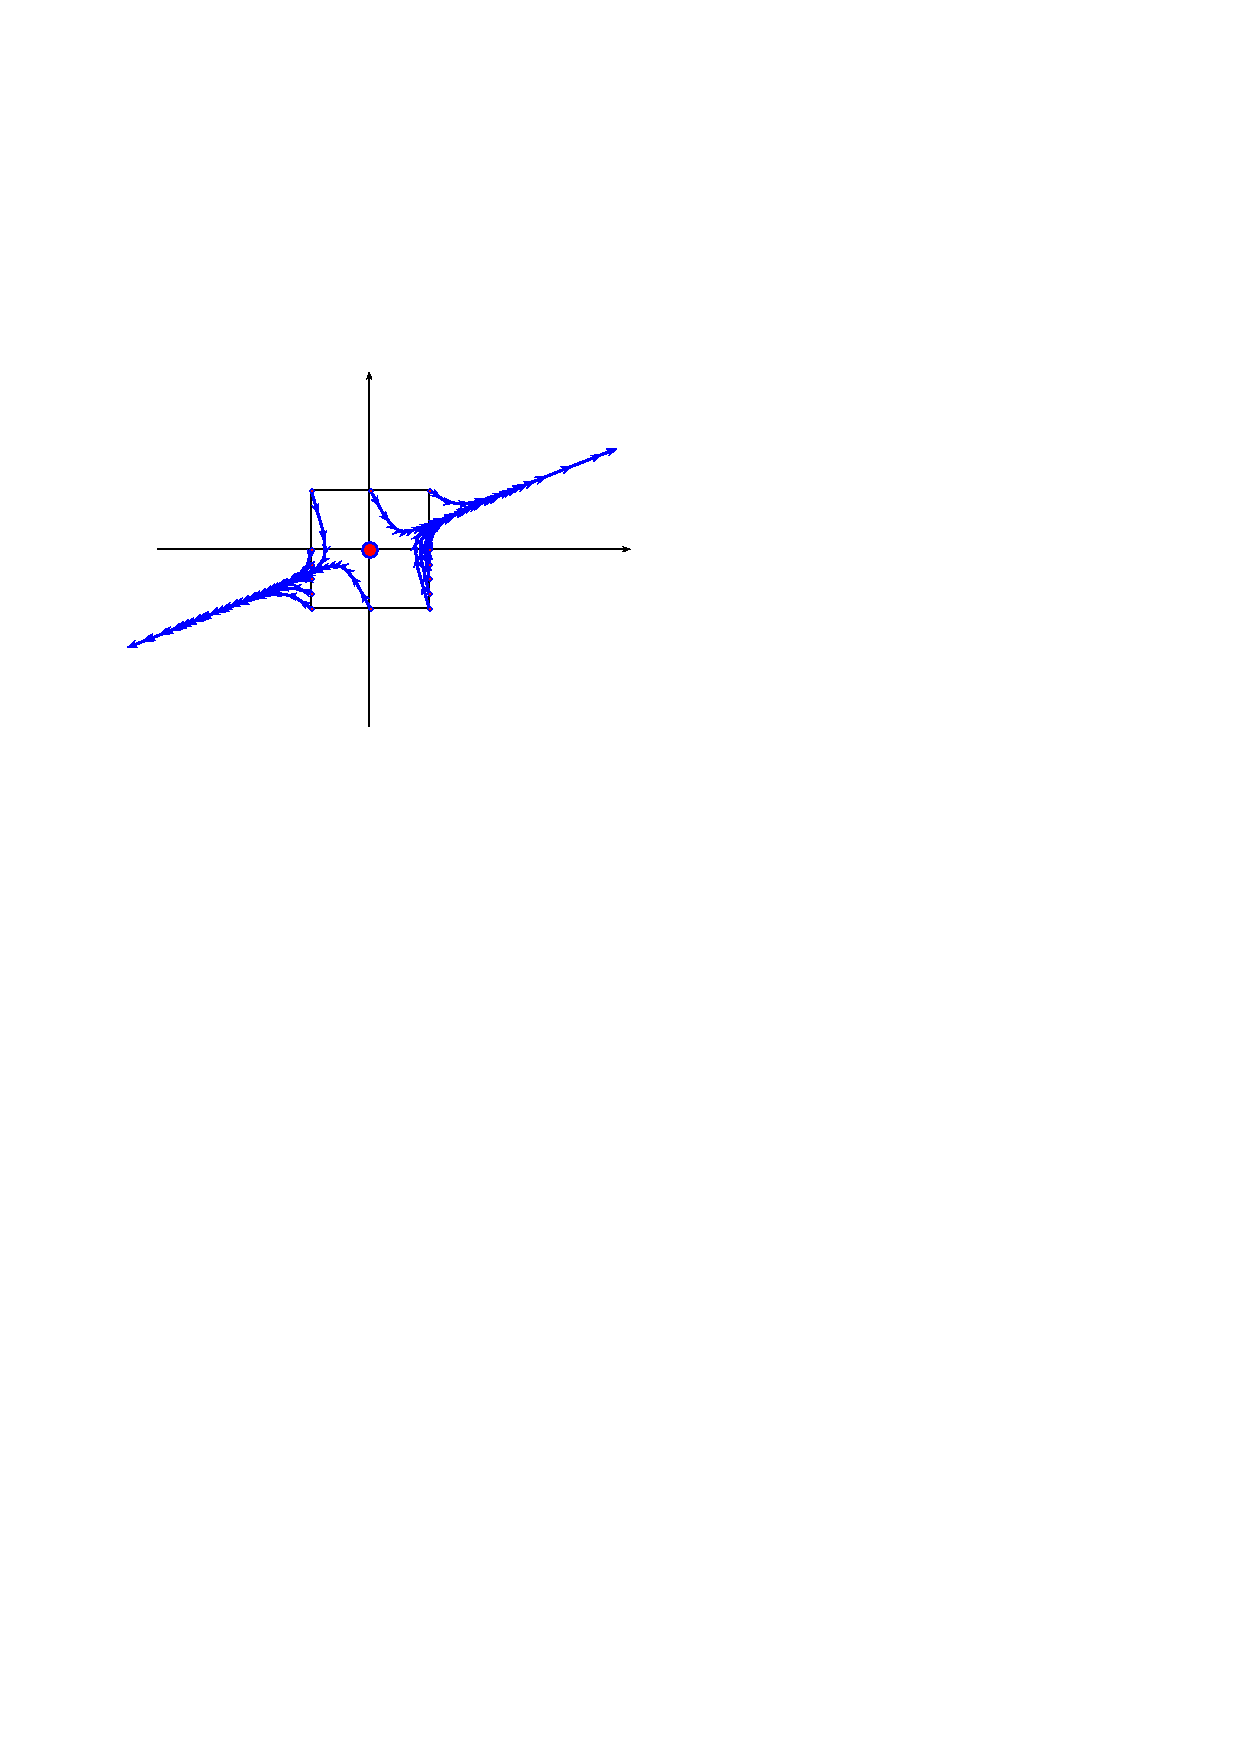
\includegraphics{unstablePosition}
    \fi
    \caption{Unstable Posture}
    \label{fig:unStablePosture}
  \end{center}
\end{figure}


\subsubsection*{''Easiness''}
If we plot all the possible motion of the ship, we get the \textbf{phase portrait} of the ship. 
We find out that all the curves will move away from the repelling posture to the attractive posture.
 Several curves are show in figure ~\ref{fig:globalflow}
\begin{figure}[!htbp]
  \begin{center}
    \leavevmode
    \ifpdf
      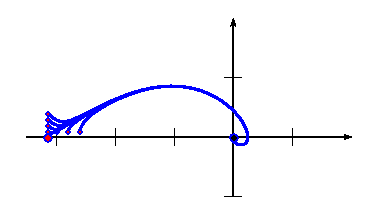
\includegraphics[height=6in]{ShipGlobalFlow}
    \else
      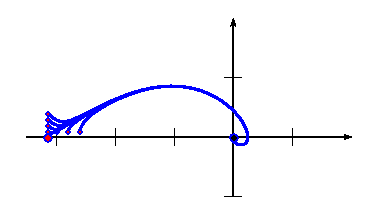
\includegraphics[width=0.7\textwidth]{ShipGlobalFlow}
    \fi
    \caption{Several Possible Motion of Ship}
    \label{fig:globalflow}
  \end{center}
\end{figure}

Thus we come to the conclusion, the ship can automatically control maintain its left equilibrium posture. 
Ship can keep its upside up as long as the centre of buoyancy force is above the centre of gravity.
Maintaining posture of the ship is very ”easy”.


\subsubsection*{Different Ships} 
Something interesting in our analysis is the conclusion is independent of the detail information about the size, weight and design of the ship. 
It is obvious different ship will maintain its posture with different motions. 
Or put in a different phrase, ship will adapt its motion during maintain posture when we change the ship  parameters.

As long as the centre of buoyancy is above the centre of gravity, maintaining posture is “easy”.
One phase plot, all the ships share some properties: one repealing point, one attractive point and all motion curves moves away the repelling point to the attractive point. As how in Figure~\ref{fig:topologyStructure}

\begin{figure}[!htbp]
  \begin{center}
    \leavevmode
    \ifpdf
      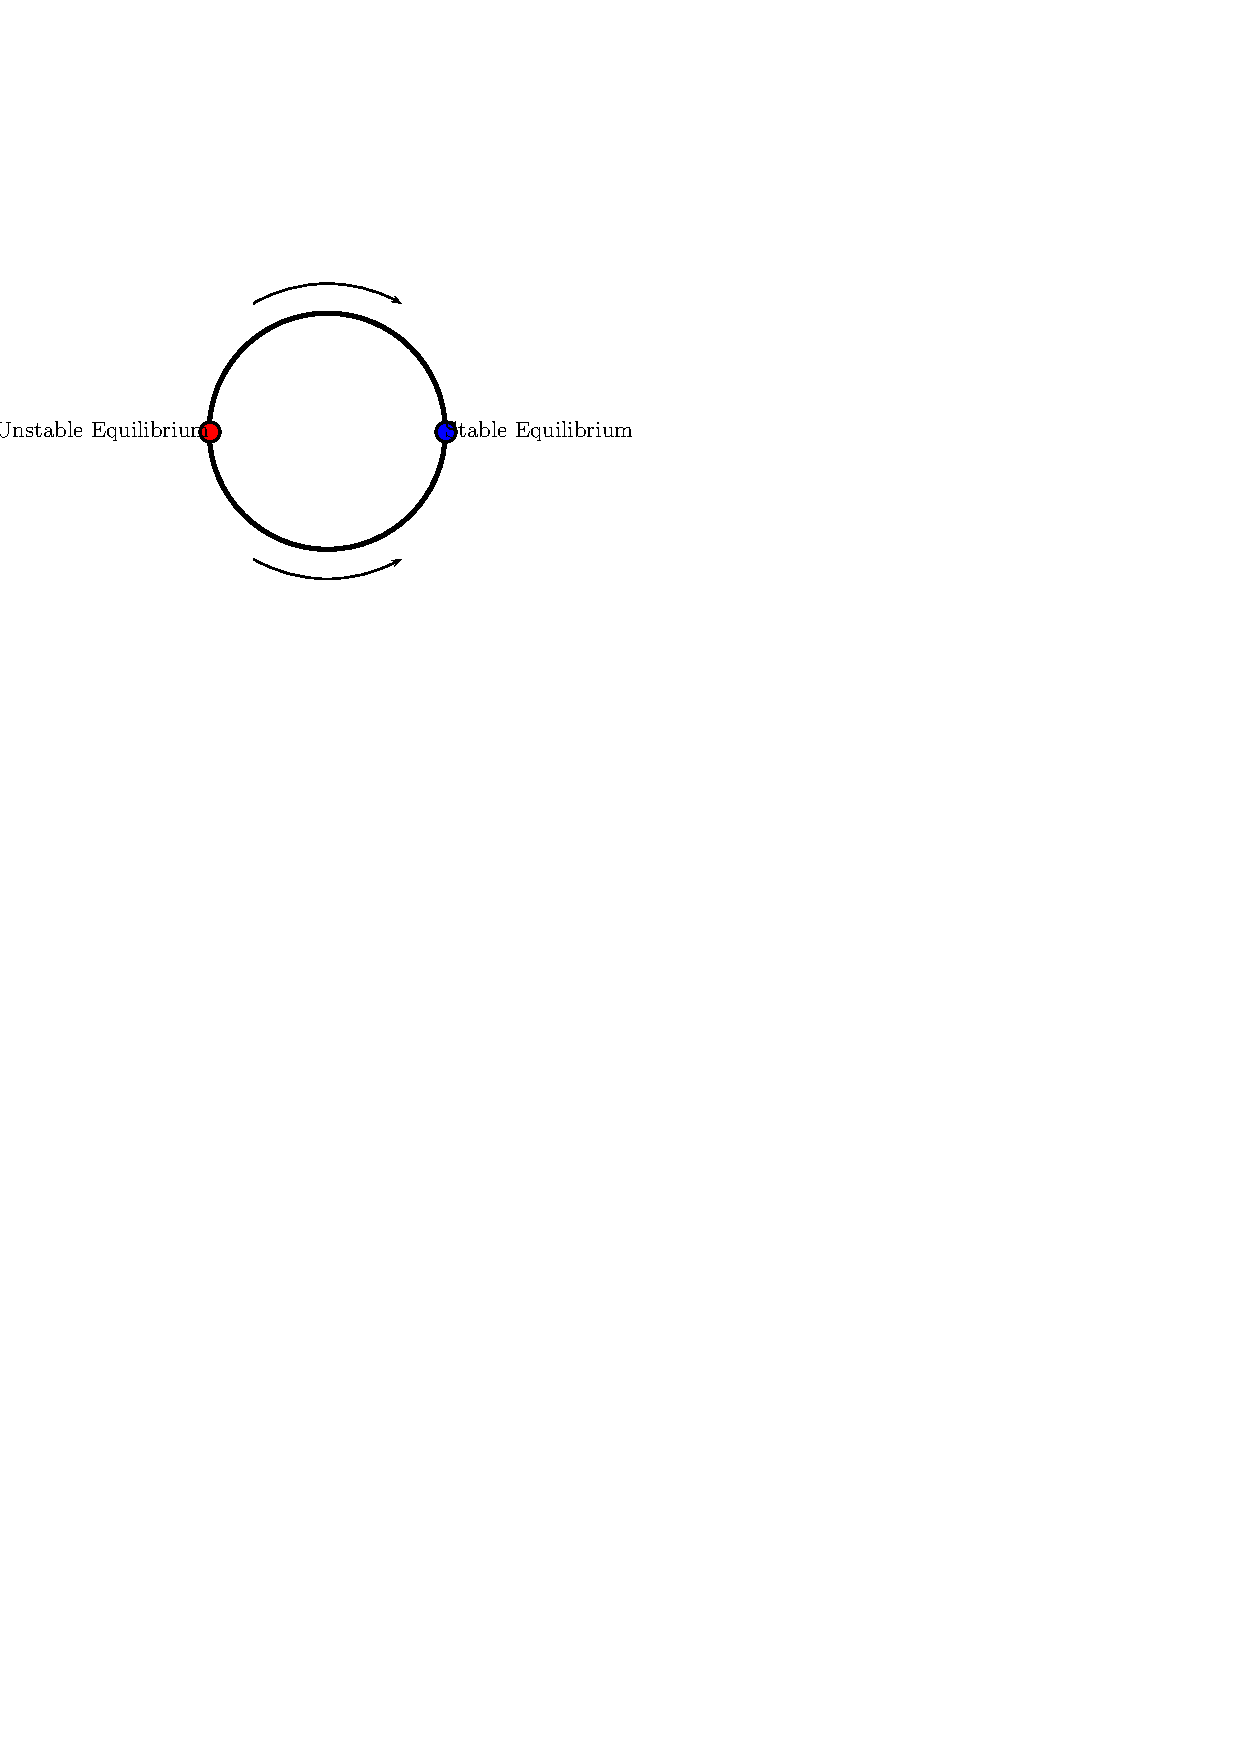
\includegraphics[height=6in]{topologyStructure}
    \else
      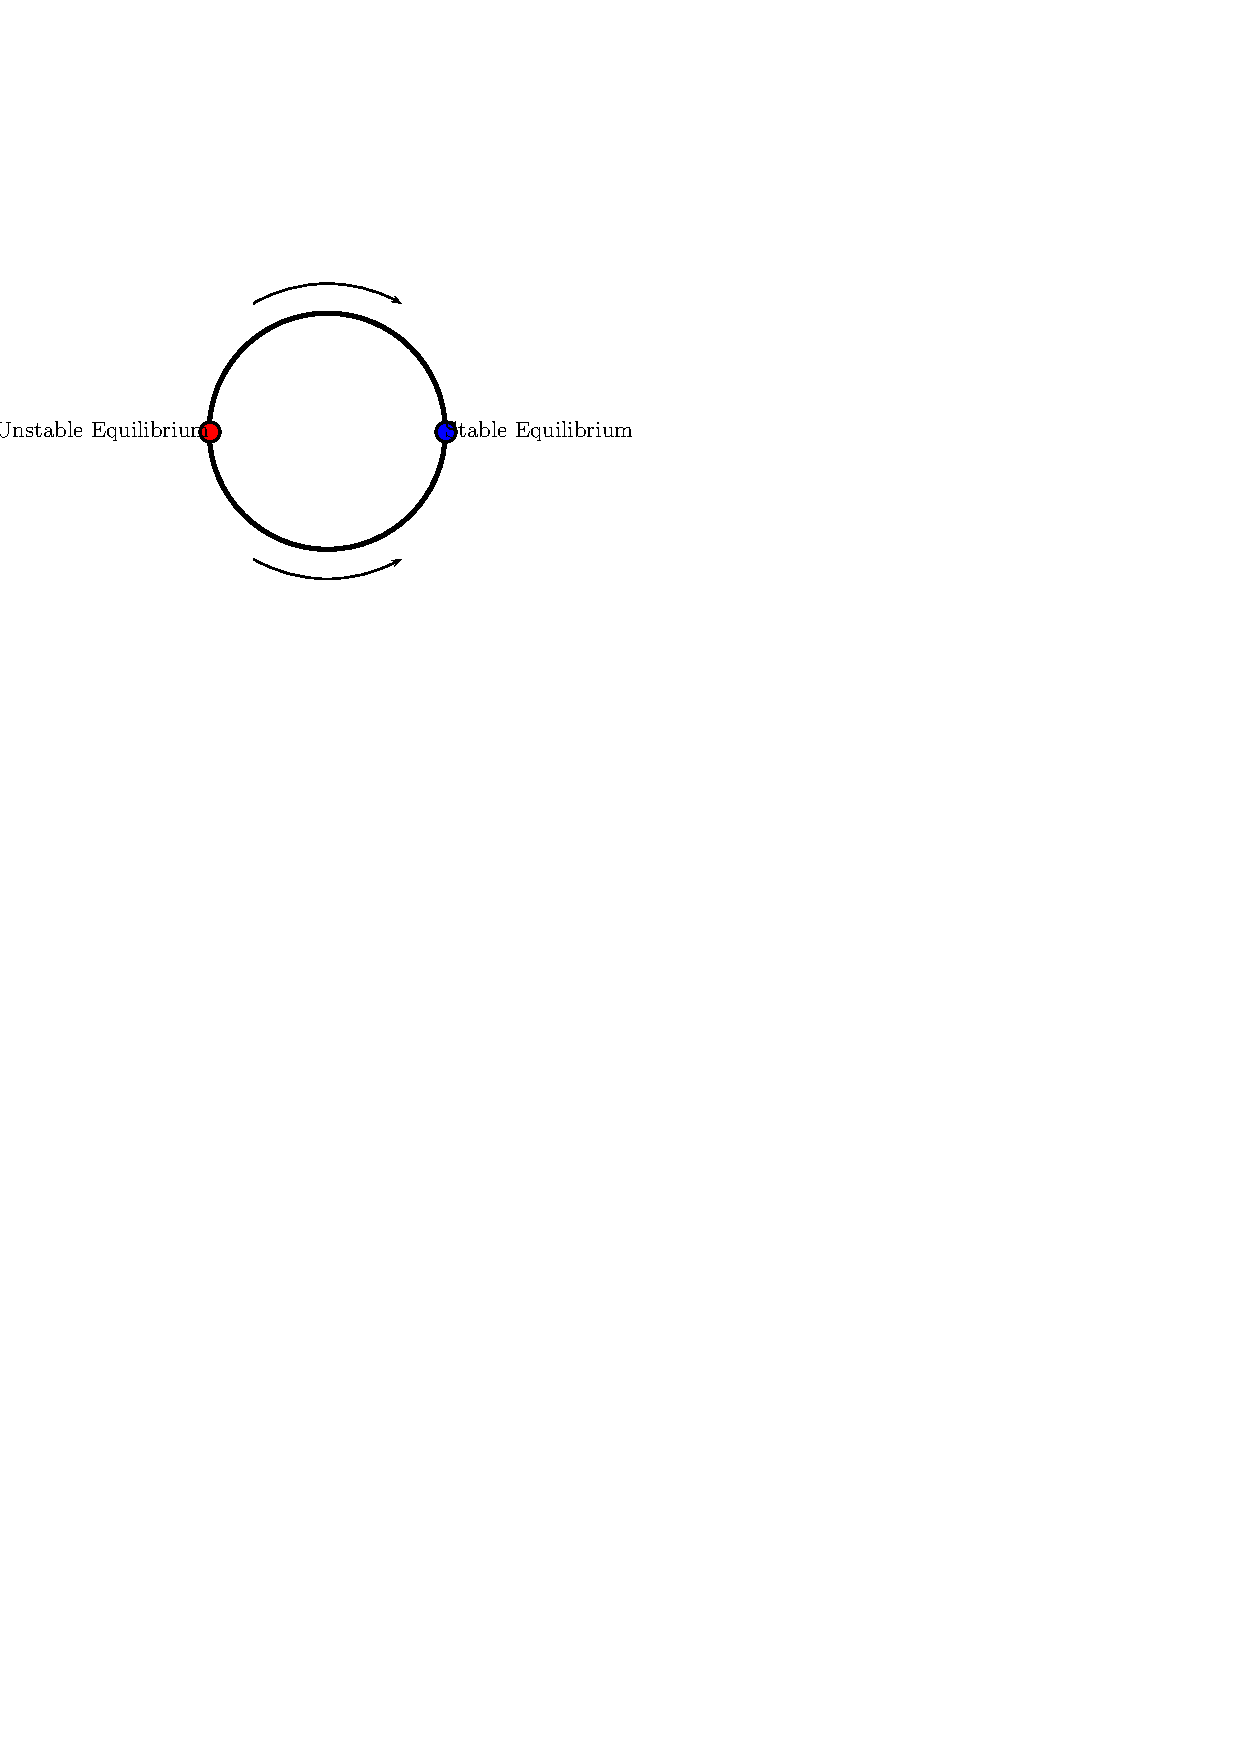
\includegraphics{topologyStructure}
    \fi
    \caption{The Topology Structure}
    \label{fig:topologyStructure}
  \end{center}
\end{figure}


Such properties are “topological property”.
As long as the topology is maintained, for different kinds of ship,maintaining posture is “easy”.

The dynamic system of two ships are presented by two equation $x=F_1(x)$ and $x_=F_2(x)$,
if they share the same topology, we can say they are topological equivalant,represent by the symbol $F_1 \simeq F_2$
this kind of relationship is \textbf{topology conjugacy}
and $F_1$ , $F_2$ are called analogous system.



\subsubsection*{Global Motor Invariant and System Adaptation}
In our motion synthesis framework, the topology is called \textbf{global invariant}, and they encapsulate the qualitative properties of a dynamic system.

For “easy” task, no control is need.
Following this idea, to find the “easy” motion task, we should investigate the topology of the phase portrait.

Another important idea is motion will adapt when we change the parameters of the dynamic system,which is called \textbf{System Adaptation}


\subsection{The Mass-Spring Vibration}
Human can finish motion tasks require high accuracy.
The question is how neural systems solve the complex dynamic problem instantly with high accuracy.
The biological motor control is very complex; it involves chemical, neural, electrical and mechanical process. 

An alternative idea is we don’t find the solution by solving the dynamics; we only need to know how to transform one solution into another.
This idea is illustrative in the following mass spring example

\subsubsection*{Dynamics}

\begin{figure}[!htbp]
  \begin{center}
    \leavevmode
    \ifpdf
      \includegraphics[height=6in]{MassSpring}
    \else
      \includegraphics[width=0.7\textwidth]{MassSpring}
    \fi
    \caption{Mass Spring}
    \label{fig:massspring}
  \end{center}
\end{figure}
Although simple, this system in Figure~\ref{fig:massspring} captures some of the important properties of motor control system.
The biological motor actuation or muscle works more like spring rather than the artificial electrical motor. 
Neural control adjusts spring rather applying force direct at the mass (which model the skeleton).


The canonical equation of mass spring system is equation (\ref{eq:mass-spring})
\begin{equation}
\label{eq:mass-spring}
\ddot{q}+q=0.
\end{equation}

In a similar manner, we can draw the state of mass spring system on the phase plot, as show in Figure~\ref{fig:massSpringPhasePlot}


\begin{figure}[!htbp]
  \begin{center}
    \leavevmode
    \ifpdf
      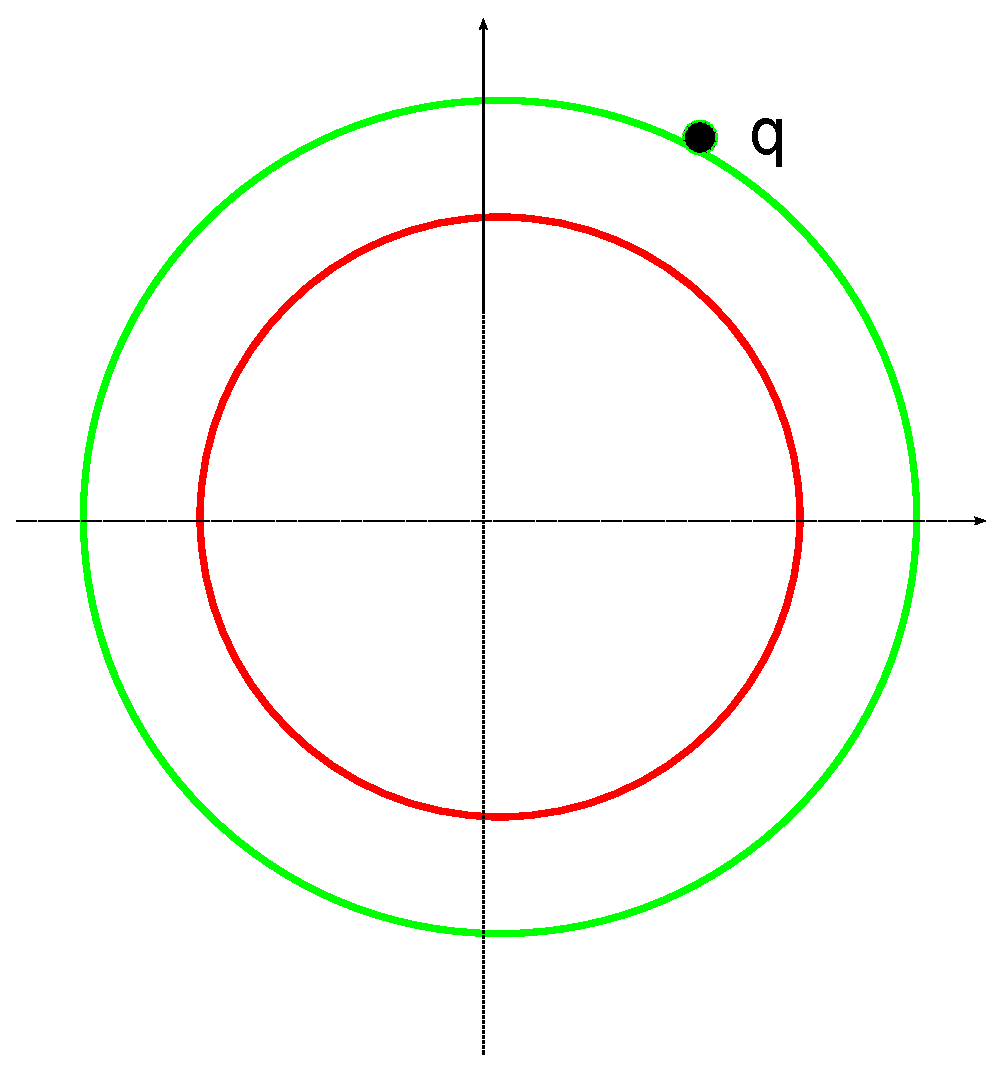
\includegraphics[height=6in]{MassSpringPhasePlot}
    \else
      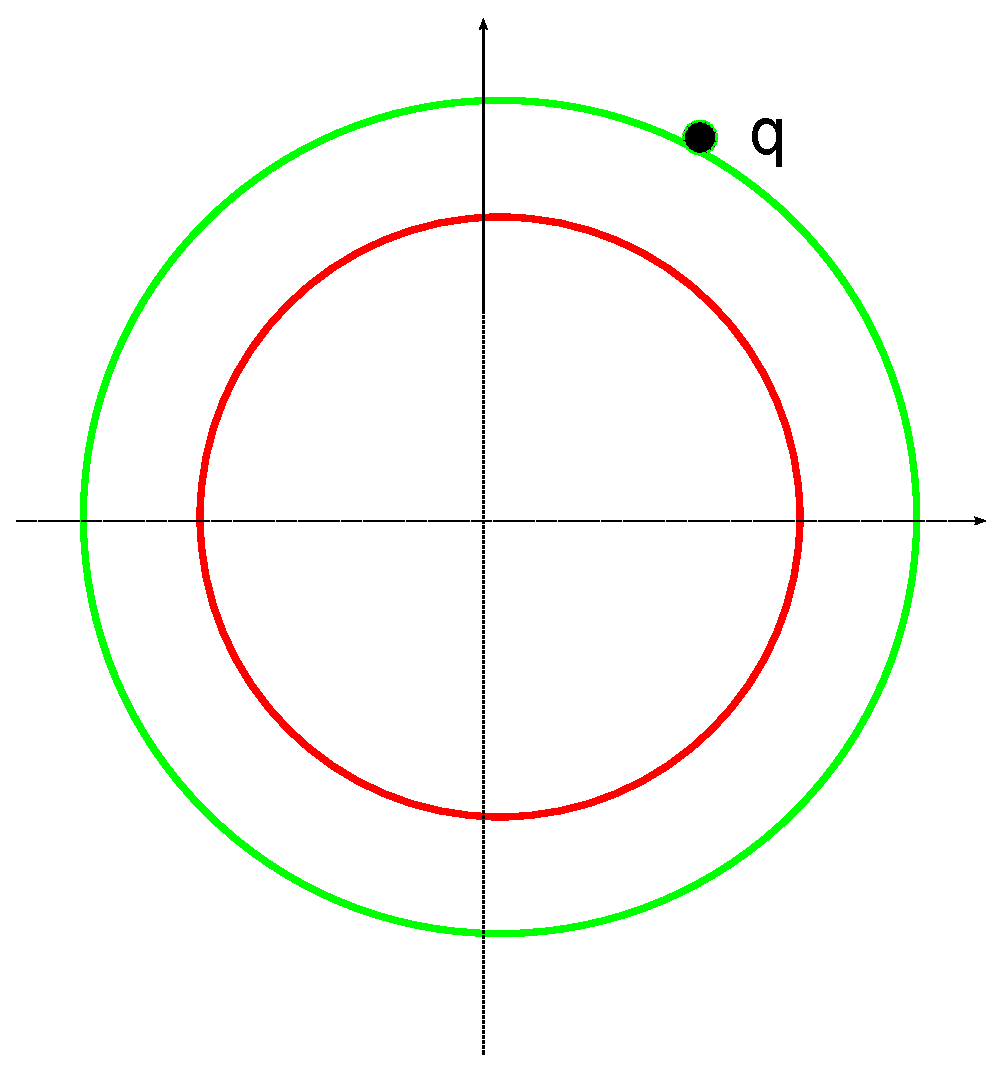
\includegraphics[width=0.5\textwidth]{MassSpringPhasePlot}
    \fi
    \caption{Mass Spring Phase Plot}
    \label{fig:massSpringPhasePlot}
  \end{center}
\end{figure}

\subsubsection*{Symmetry and Transformation}
Even it is simple, it is highly unlikely the knowledge of the mass spring is encoded in our brain in the form of equation (\ref{eq:mass-spring}).
Very possible we know a possible motion like the red one.
 Given a state $[q,\qd]$, we can easily work out the motion curve, it is on the green circle that shares the centre with the red one, but has a bigger radius.
 We can say the green curve is a scale red curve.
 The property that we can transform one motion into another is called ''symmetry''.

Using transformation, the new motion can be calculated easily.
In fact we can ignore the complexity of the dynamic system, as long as we know the ''symmetry'' property of a dynamic system. 
Given one motion, we can work out all the possible motions.

\subsubsection*{Dynamic Encoding}

The dynamic system can be encoded in a different manner,a possible way is store a motion curve and its symmetrical property.

Impact of this idea for motor control is far reaching. 
\begin{itemize}
\item it greatly reduces the computational cost in motor control.
\item It also provides us with an idea of motion perception. 
In fact we don’t calculate the details dynamic of motion; we can check the ''symmetry''.
If we can transformed the observed motion(green) into our memorized one (red), than we think the motion are realistic, otherwise we detect artefacts.
\end{itemize}

\subsubsection*{Local Motor Invariant and Transform Adaption}
When comparing the observed motion and the memorized motion, there is a better method than work out the transformation directly. 
Some property should be kept invariant under such transformation, for the mass spring system, we can say the shape is kept during scale transformation. 
From Differential Geometry view port, we can say the curvature is kept. 
From mechanical view, we can say for each motion, the energy is kept along the curve, and different motion is of different energy. 

Energy and Curvature are called \textbf{Local Invariant.} 
And the transformation from one motion to another motion is called \textbf{transform adaptation}.

\section{Contribution}




\section{Overview of the Thesis}
Global Motor Invariant contains the qualitative properties while Local Motor Invariant contains quantitative properties. 
For our motion synthesis method, the design idea is to keep the both motor invariants. 
Motion Adaptation is achieved through System adaptation(change system parameters) and Transform Adaptation.
In application, this method easy to compute and result realistic motion adaptation.



This thesis is organized as follows.
 
In Chapter~\ref{chap:background}, we will discuss some previous research work of motion synthesis  and biological motor control. 
These are the motivation and justification of our ideas.
 
In Chapter~\ref{chap:gi}, we will focus on the Global Motor Invariant. 
We try to identify the qualitative properties of motion and investigate method maintaining the global motor invariant based on some biological ideas.

In Chapter~\ref{chap:li}, we discuss on the idea of Local Motor Invariant and Symmetry.
Mathematical tools are developed and we show how to apply control effort to ensure symmetry. 
We show the computational complexity is greatly reduced by symmetry.

In Chapter~\ref{chap:msf}, we discuss how the Global Motor Invariant and Local Motor Invariant Controller work together. 
Simple example is included to discuss the mathematical idea. 
Also we give an idea about how to connect motion primitives together to form more complex motion behaviour.

Chapter ~\ref{chap:gi},\ref{chap:li},\ref{chap:msf} lay the theory foundation for the motion synthesis control and be treated as the Motion Invariant Theory.


In Chapter~\ref{chap:walk}, we focus on synthesizing motion of one motion primitives
 we apply our method for one of the most interesting and challenging motion synthesis research topic, bipedal walking. We show how our method main the stability and adaptive to different walking situation.


In Chapter ~\ref{chap:stance}, we will discuss how to connecting motion primitives together.
New Motion Primitives (the balancing) is developed. We show how we an approximate with discrete motion with periodic motion. We show how different motion primitives connected together by switching the motion from stance to walk and from walk to stance.

In Chapter ~\ref{chap:highdor}, we discuss about extend the basic idea to more complex system, or scale our method to address system with more difficult motion tasks. Three possible ideas discussed are the reduction, mechanical coupling and ad-hoc manner. The three ideas apply to different types of biomechanical system.
Hopefully they will help us to synthesis motion we have not achieved yet.

In Chapter 9, we will discuss about some future work. After a retrospective discussion, we proposed some new question and ideas for graphics and neural science for further research.





%%% ----------------------------------------------------------------------


%%% Local Variables: 
%%% mode: latex
%%% TeX-master: "../thesis"
%%% End: 

